\InputIfFileExists{../data/global.src}\relax\relax

\iffull
\setbox\pinguA=\hbox{\tikz\marmot[whiskers=gray,shadow];}\relax
\titlesuffix{\tikzpicture[@O]
    \node[above left,yshift=\btdmfootheight] at(current page.south east) {\copy\pinguA};
\endtikzpicture}

\title{Täglich grüßt das Murmeltier!} % \ldots\ sich selbst
\subtitle{Tutorium sieben}
\date{KW 25}
\addbibresource{references.bib}
\fi
\SetTutoriumNumber{7}

\iffull\begin{document}
\titleframe

\TopicOverview{7}
\fi

\iffull{\SummaryFrame
\begin{frame}[c]{Kurzwiederholung}
\begin{itemize}[<+(1)->]
   \itemsep14pt
   \item Eine Methode die sich selbst aufruft heißt rekursiv \begin{itemize}
    \item Die Rekursion ist linear, wenn sie sich maximal einmal selbst aufruft
    \item Solche sind \say{End-Rekursiv}, wenn der Aufruf das letzte ausgeführte Statement ist
    \item Rekursion und Iteration sind dabei gleichmächtig
   \end{itemize}
   \item Damit wir Bezeichner verwenden können müssen diese gültig und sichtbar sein \begin{itemize}
        \item Die Gültigkeit hängt an der Deklaration (Überschattung,~\ldots)
        \item Die Sichtbarkeit hängt an Modifikatoren wie \bjava{public}, \bjava{private},~\ldots
   \end{itemize}
   \item Methoden haben Seiteneffekte, wenn sie den Programmzustand über den Rückgabewert hinaus verändern
   \begin{itemize}
    \item Seiteneffekte sind ein großes Problem und sollten erstmal vermieden werden
    \item Ganz ohne geht es allerdings nicht (Konsolenausgaben,~\ldots)
   \end{itemize}
\end{itemize}
\end{frame}
}\fi

% TODO: make sectionlink auto triggerat start of section
\SetNextSectionText[.75\linewidth]{TODO}
\section{Präsenzaufgabe}
{\taskenum
\begin{frame}[fragile,c]{Präsenzaufgabe}
\begin{aufgabe}{Irgendwo sind meine Socken doch}
\task<2->{In der Vorlesung wurde der Binary Algorithmus zur Suche in einer geordneten Struktur vorgestellt. \begin{enumerate}[<+(1)->]
    \item Geben Sie an, wie das folgende Array vom Suchalgorithmus Binary Search nach dem Schlüssel \say{4} durchsucht wird.
    \begin{center}
        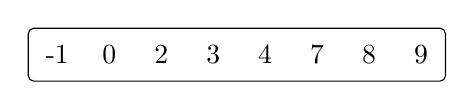
\begin{tikzpicture}
            \foreach[count=\i from 0] \a in {-1,0,2,3,4,7,8,9} {
                \node[outer sep=3pt] (\a) at (.66*\i, 0) {\a};
            }
            \draw[rounded corners=2pt] (-1.south west) rectangle (9.north east);
        \end{tikzpicture}
    \end{center}
    \item Begründen Sie \textit{kurz}, weshalb der Binary Search Algorithmus eine worst-case Laufzeit von \(T(n)_{max} \in \O(\log n)\) hat.
\end{enumerate}}
\end{aufgabe}
\end{frame}
}

\begin{frame}[c]{Ja wie suchen wir denn die 4?}
\begin{center}
    \onslide<2->{\begin{tikzpicture}
        \foreach[count=\i from 0] \a/\ao/\ho/\co in {-1/2/0/{6-|handout:2-},0/2/0/{6-|handout:2-},2/2/0/{6-|handout:2-},3/{2,3,4,5}/1/{6-|handout:2-},4/{2,3,9,10}/3/{0|handout:0},7/{2,6,7,8}/2/{9-|handout:3-},8/{2,6}/0/{9-|handout:3-},9/2/0/{9-|handout:3-}} {
            \color{gray}\only<\ao|handout:\ho>{\color{black}}
            \expandafter\only\expandafter<\co>{\color{codeouthl}}
            \node[outer sep=3pt] (\a) at (.66*\i, 0) {\a};
            \node[below=2mm,codeouthl,font=\footnotesize\sffamily] (\a-i) at(\a.south) {\i};
        }
        \draw[rounded corners=2pt] (-1.south west) rectangle (9.north east);
        \onslide<3|handout:0>{\path(3-i.north)--(4-i.north) coordinate[pos=.5] (@); \node[above=-2mm] at(@.north) {\faAngleUp};}
        \onslide<4-5|handout:1>{\node[above=-2mm] at(3-i.north) {\faAngleUp};}
        \onslide<5|handout:1>{\node[above=2mm] at(3.north) {\(3 < 4\)};}
        \onslide<6|handout:0>{\path(7-i.north)--(8-i.north) coordinate[pos=.5] (@); \node[above=-2mm] at(@.north) {\faAngleUp};}
        \onslide<7-8|handout:2>{\node[above=-2mm] at(7-i.north) {\faAngleUp};}
        \onslide<8|handout:2>{\node[above=2mm] at(7.north) {\(7 > 4\)};}
        \onslide<9-10|handout:3>{\node[above=-2mm] at(4-i.north) {\faAngleUp};}
        \onslide<10|handout:3>{\node[above=2mm] at(4.north) {\(4 = 4\)};}
    \end{tikzpicture}}
\end{center}
\begin{onlyenv}<0|handout:1->
\begin{enumerate}
    \itemsep7pt
    \setcounter{enumi}{-1}
    \item<handout:1-> Initial ist \(\text{min = 0}\) und \(\text{max = 7}\). Wir springen in die Mitte: \(\text{mid} = \floor{(\text{min} + \text{max})/2}\). \infoblock{Hierbei runden wir im Gleichheitsfall ab. Das ist an sich willkürlich, hier aber von uns festgesetzt.}
    \item<handout:1-> Das betrachtete Element ist kleiner als der Schlüssel, wir springen in die rechte Hälfte.\infoblock{Das heißt wir verschieben \(\text{min} = \text{mid} + 1\) und wiederholen die Berechnung von \(\text{mid}\).}
    \item<handout:2-> Das betrachtete Element ist größer als der Schlüssel, wir springen in die linke Hälfte. \infoblock{Das heißt wir setzen \(\text{max} = \text{mid} - 1\) und wiederholen die Berechnung von \(\text{mid}\).}
    \item<handout:3> Das betrachtete Element entspricht dem gesuchten, liefere Index: \(4\) zurück.
\end{enumerate}
\end{onlyenv}
\begin{tikzpicture}[@O]
    \node[below left,yshift=-1.35cm,align=left] at(current page.north east) {\only<3-|handout:1->{\(\frac{0+7}{2} = 3.5 \onslide<4->{\rightarrow 3}\)}\\[1.5mm]\only<6-|handout:2->{\(\frac{4+7}{2} = 5.5 \onslide<7->{\rightarrow 5}\)}};
\end{tikzpicture}
\end{frame}

\begin{frame}{Und warum ist das schnell?}
    \begin{itemize}[<+(1)->]
        \itemsep10pt
        \item Mit jedem Vergleich sind wir entweder fertig, oder wir halbieren den Suchraum
        \item Bei \(n\) Elementen können wir maximal \(\log_2(n)\) oft halbieren \infoblock{Ist \(n = 8\) so beispielsweise \(\log_2(8) = 3\) mal.}
        \item So benötigen wir maximal \(\log_2(n)\) viele Vergleichsschritte
        \item Bei der \(\O\)-Notation ist die Basis des Logarithmus egal\infoblock{So ist für \(\log_a(x)\) der Unterschied zu \(\log_b(x)\) nur ein Faktor, der sich durch den Basiswechsel ergibt. Es ist: \(\log_a(x) = \frac{\log_b(x)}{\log_b(a)}\) dabei ist \(\log_b(a)\) eine Konstante die von der \(\O\)-Notation verschluckt wird.}
        \item So kommen wir auf \(\O(\log n)\)
    \end{itemize}
\end{frame}

\SetNextSectionText{Grundlagen der Rekursion\\Abgabe: \DTMDate{2022-06-20}}
\section{Übungsblatt 7}
\subsection{Aufgabe 1}
{\taskenum
\begin{frame}[fragile,c]{Aufgabe 1: Ablauf eines rekursiven Programms}
    \task<2->{Für einen rekursiv definierten Algorithmus kann man ein \say{Berechnungsformular} aufstellen, das für jeden rekursiven
    Aufruf (Inkarnation) vervielfältigt wird. Das Ergebnis der Berechnung wird dann durch Ein- und Rückübertragung
    von (Teil-) Lösungen bestimmt, wobei die Termination durch die Reduktion des Arguments ausgelöst wird. In dieser
    Aufgabe sollen Sie eine derartige Formularmaschine selbst angeben.

    \onslide<3->{Betrachten Sie das folgende rekursive Programm und geben Sie das Formularblatt, sowie die Inkarnationen für den Aufruf \T{ggt(6, 3)} an. Folgen Sie dabei der Gestaltung und Ausführung des Beispiels aus der Vorlesung (Kap.~8, Folien 15ff.)}}
    \begin{plainjava}
!*\onslide<4->*!public int ggT(int a, int b) {
!*\onslide<4->*!    if(b == 0) {
!*\onslide<4->*!        return a;
!*\onslide<4->*!    } else {
!*\onslide<4->*!        return ggt(b, a % b);
!*\onslide<4->*!    }
!*\onslide<4->*!}
    \end{plainjava}
\end{frame}
}

\begin{frame}[c,fragile]{Formulargefahr}
\begin{onlyenv}<3-|handout:1>
\raisebox{-.5\height}{\begin{forest}
   for tree={inner sep=4pt,block,minimum width=2em,outer sep=1pt,execute at begin node={\strut},grow=north}
   [{},label=left:ggT[6,label=right:a][3,label=left:b]]
   \node[above right] at(current bounding box.north west) {Initialer Aufruf};
\end{forest}}$\equiv$\raisebox{-.5\height}{\begin{forest}
    for tree={inner sep=4pt,block,minimum width=2em,outer sep=1pt,execute at begin node={\strut},grow=north}
    [{},label=left:if[false,label=right:{=}[6,label=right:b][0]][6,label=above:b][\paletteA{?},label=left:ggT[3][0[6][3]]]]
    \node[above right] at(current bounding box.north west) {Inkarnation \(1\): \(a = 6\), \(b = 3\)};
    % TODO:animationen von unten ncach oben und andere steps mit handout breakds, bei der zwei einfach nur sperat animieren wie die aufploppenund bei der drei mehr reden als auf die FOlien packen (vielleicht einn QR code zum numberphile video oder so....)
 \end{forest}}
\end{onlyenv}
\begin{tikzpicture}[@O]
\begin{onlyenv}<2->
\node[below left,yshift=-1.35cm,text width=5.25cm] at(current page.north east) {\lstfs{9}\begin{plainjava}
public int ggT(int a, int b) {
    if(b == 0) {
        return a;
    } else {
        return ggt(b, a % b);
    }
}
    \end{plainjava}};
\end{onlyenv}
\end{tikzpicture}
\end{frame}

\iffull
\SetNextSectionText{Suchen und Sortieren\\Abgabe: \DTMDate{2022-06-27}}
\section{Aussicht: Übungsblatt 8}
\begin{frame}{Habbeldu}
\end{frame}
\fi

\SetNextSectionText[.55\linewidth]{TODO}
\section{Abschließendes}
{\SummaryFrame
\begin{frame}[t]{Zusammenfassend}
\pause \printBibCommand
\vfill\vfill % double fill for more fraction
\begin{itemize}[<+(1)->]
    \itemsep5pt
    \item TODO
\end{itemize}
\end{frame}
}

\outro{\vskip9mm\centering \onslide<2->{\scalebox{1.35}{\begin{tikzpicture}
       % TODO
\end{tikzpicture}}}}

\iffull\end{document}\fi
